\documentclass[12pt,letterpaper]{exam}

\usepackage[left=2cm,top=2cm,right=2cm,bottom=2.5cm]{geometry}
\usepackage{hyperref}
\usepackage[utf8]{inputenc}
\usepackage[spanish,activeacute]{babel} % Escribir en español
\decimalpoint
\usepackage{enumerate}
\usepackage{eurosym}
\usepackage{latexsym,amsmath,amsthm,amssymb,amsfonts,bbm, dsfont}
\usepackage[mathscr]{euscript}
\usepackage{ae,aecompl}
% \usepackage{pdflscape}

% --- Imágenes y colores ---
\usepackage{graphicx}
\DeclareGraphicsExtensions{.pdf,.png,.jpg}
\usepackage{adjustbox}
\usepackage[dvipsnames]{xcolor}

%---- modificar las caption -----
\usepackage[font=small,labelfont=small,labelfont=bf,textfont=it]{caption}
\usepackage{enumitem}
\usepackage{float}
\usepackage{subfigure}
\usepackage{multirow}
\usepackage{fancybox}

% === RUTAS DE APOYO (opcional; no dependemos de esto para las tablas) ===
\graphicspath{{../assets/}{../Talleres_fundamentos/}{./}}


%--------------------------------------------------------------------
\newcommand{\base}[1]{\underline{\hspace{#1}}}
%--------------------------------------------------------------------
\newcommand{\uni}{Universidad Sergio Arboleda}
\newcommand{\fac}{\normalsize{Escuela de Ciencias Exáctas e Ingeniería}}
\newcommand{\dep}{Matemáticas}
\newcommand{\mat}{Fundamentos de  Matem\'aticas} %Materia
\newcommand{\tema}{} %Tipo y Número de Quiz
\newcommand{\autor}{Adriana M. Salinas}
%\newcommand{\fecha}{\textbf{Duración}: 100 minutos}
\newcommand{\espacio}[1]{\vspace{#1}}

%---------------------------------------------------------------------
\pagestyle{headandfoot}
\footrule
\headrule
\firstpageheader{}{}{}
\firstpagefooter{}{\thepage $\,$ de \numpages}{}
\runningfooter{\uni}{\thepage $\,$ de \numpages}{}

\begin{document}

% ===== Encabezado institucional =====
\begin{tabular}{lr}
    \multirow{2}{*}{
\includegraphics[height=1.4cm]{logosergio.png}} &
    {\textbf{\uni}} \\
    & {\textbf{\fac}} \\
    & {\textbf{\dep}} \\
    & {\textbf{\mat \tema}} \\
    & {\textit{\autor}} \\
    & {\textit{}}
\end{tabular}\\
\base{19.5cm}\\
% \textbf{Nombre}: \base{13.2cm} \quad \textit{Calificación}: \base{2cm} \\[6pt]
\textbf{Nombre}: \makebox[11.2cm]{\hfill Juan Sebastioan Ladino Mendieta \hfill} \quad 
\textit{Calificación}: \base{2cm} \\[6pt]
% ===== TALLER 1 =====
\section*{Taller 1}

\begin{enumerate}
  \item Determine si se trata de una proposición o no.
  \begin{enumerate}[label=\alph*)]
    \item El 2 de febrero de 2009 fue lunes. \textcolor{ForestGreen}{Proposición.}
    \item El código postal de Óscar, en Los Ángeles, es 70762. \textcolor{ForestGreen}{Proposición.}
    \item Ceda el paso al tráfico en sentido contrario. \textcolor{red}{No es proposición.}
    \item $5+9 \neq 14$ y $4-1=12$. \textcolor{ForestGreen}{Proposición.}
    \item Algunos números son positivos. \textcolor{ForestGreen}{Proposición.}
    \item \textit{The Dark Knight} (El caballero de la noche) fue la película que logró mayor recaudación en 2008. \textcolor{ForestGreen}{Proposición.}
    \item ¿A dónde vas a ir mañana? \textcolor{red}{No es proposición.}
    \item Compórtate y siéntate. \textcolor{red}{No es proposición.}
  \end{enumerate}

  \item Indique si los enunciados son compuestos o no.
  \begin{enumerate}[label=\alph*)]
    \item Mañana es sábado. \textcolor{red}{No es compuesto.}
    \item Las flores se van a regar. \textcolor{red}{No es compuesto.}
    \item Ningún técnico de computadoras puede jugar blackjack. \textcolor{red}{No es compuesto.}
  \end{enumerate}

  \item Dé una negación para cada desigualdad. No use el símbolo con la diagonal.
  \begin{enumerate}[label=\alph*)]
    \item $x>12$ \; su negación es: \; $\neg(x>12)\ \rightarrow\ x\leq 12$.
    \item $x<-6$ \; su negación es: \; $\neg(x<-6)\ \rightarrow\ x\geq -6$.
    \item $x\geq 5$ \; su negación es: \; $\neg(x\geq 5)\ \rightarrow\ x<5$.
    \item $x\leq 19$ \; su negación es: \; $\neg(x\leq 19)\ \rightarrow\ x>19$.
  \end{enumerate}

  \item Considere que $p$ representa el enunciado “Ella tiene ojos verdes”, mientras que $q$ representa “Ella tiene 60 años”. Convierta a palabras cada enunciado simbólico.
  \begin{enumerate}[label=\alph*)]
    \item $\neg p$: No ocurre que ella tiene ojos verdes.
    \item $\neg q$: No ocurre que ella tiene 60 años.
    \item $p \lor q$: Ella tiene ojos verdes o ella tiene 60 años.
    \item $p \land q$: Ella tiene ojos verdes y ella tiene 60 años.
    \item $\neg p \lor q$: No ocurre que ella tiene ojos verdes o ella tiene 60 años.
    \item $\neg p \land q$: No ocurre que ella tiene ojos verdes y ella tiene 60 años.
    \item $p \lor \neg q$: Ella tiene ojos verdes o no ocurre que ella tiene 60 años.
    \item $p \land \neg q$: Ella tiene ojos verdes y no ocurre que ella tiene 60 años.
    \item $\neg p \lor \neg q$: No ocurre que ella tiene ojos verdes o no ocurre que ella tiene 60 años.
    \item $\neg p \land \neg q$: No ocurre que ella tiene ojos verdes y no ocurre que ella tiene 60 años.
    \item $\neg(p \lor \neg q) \equiv \neg p \land q$: No ocurre que ella tiene ojos verdes y ella tiene 60 años.
  \end{enumerate}

  \item Remítase a los grupos de ilustraciones identificados como A, B, C; identifique con una letra el grupo o
  grupos que satisfacen los enunciados.

  \begin{center}
    % Usa la extensión explícita
    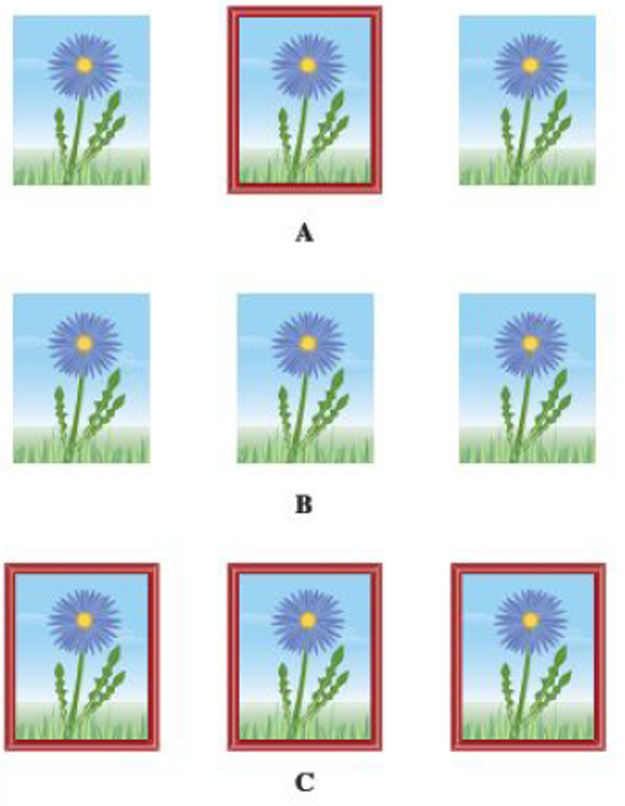
\includegraphics[width=0.3\textwidth]{../assets/Talleres_fundamentos/Taller1_imagen1.png}
  \end{center}

  \begin{enumerate}[label=\alph*)]
    \item Todas las pinturas tienen marcos. \textcolor{ForestGreen}{C}
    \item Ninguna pintura tiene marco. \textcolor{ForestGreen}{B}
    \item Al menos una pintura no tiene marco. \textcolor{ForestGreen}{A y B}
    \item No todas las pinturas tienen marco. \textcolor{ForestGreen}{A y B}
    \item Al menos una pintura tiene marco. \textcolor{ForestGreen}{A y C}
  \end{enumerate}

  \newpage

  \item Demuestre que todas las siguientes proposiciones son tautologías:

\begin{enumerate}[label=\arabic*., itemsep=-2em, topsep=0.2em]
  \item $(p \lor p) \Leftrightarrow p,\quad (p \land p) \Leftrightarrow p.$
  \begin{center}
    \adjincludegraphics[max width=\linewidth,max height=.6\textheight,keepaspectratio]{../assets/Talleres_fundamentos/tabla_01.png}\\[0.5em]
    \adjincludegraphics[max width=\linewidth,max height=.6\textheight,keepaspectratio]{../assets/Talleres_fundamentos/tabla_02.png}
  \end{center}

  \item $p \lor q \Leftrightarrow q \lor p.$
  \begin{center}
    % Si prefieres no repetir la 02 aquí, cambia a tabla_03.png
    \adjincludegraphics[max width=\linewidth,max height=.75\textheight,keepaspectratio]{../assets/Talleres_fundamentos/tabla_02.png}
  \end{center}
\newpage
  \item $(p \lor q) \lor r \Leftrightarrow p \lor (q \lor r).$
  \begin{center}
    \adjincludegraphics[max width=\linewidth,max height=.75\textheight,keepaspectratio]{../assets/Talleres_fundamentos/tabla_03.png}
  \end{center}

  \item $p \land (q \lor r) \Leftrightarrow (p \land q) \lor (p \land r).$
  \begin{center}
    \adjincludegraphics[max width=\linewidth,max height=.75\textheight,keepaspectratio]{../assets/Talleres_fundamentos/tabla_04.png}
  \end{center}
\newpage
  \item $\neg(p \land q) \Leftrightarrow (\neg p \lor \neg q).$
  \begin{center}
    \adjincludegraphics[max width=\linewidth,max height=.75\textheight,keepaspectratio]{../assets/Talleres_fundamentos/tabla_05.png}
  \end{center}

  \item $(p \land q) \land r \Leftrightarrow p \land (q \land r).$
  \begin{center}
    \adjincludegraphics[max width=\linewidth,max height=.75\textheight,keepaspectratio]{../assets/Talleres_fundamentos/tabla_06.png}
  \end{center}
\newpage
  \item $(p \land q) \land p \Leftrightarrow p \land q.$
  \begin{center}
    \adjincludegraphics[max width=\linewidth,max height=.75\textheight,keepaspectratio]{../assets/Talleres_fundamentos/tabla_07.png}
  \end{center}

  \item $p \lor (q \land r) \Leftrightarrow (p \lor q) \land (p \lor r).$
  \begin{center}
    \adjincludegraphics[max width=\linewidth,max height=.75\textheight,keepaspectratio]{../assets/Talleres_fundamentos/tabla_08.png}
  \end{center}
\newpage
  \item $p \land (q \lor r) \Leftrightarrow (p \land q) \lor (p \land r).$
  \begin{center}
    \adjincludegraphics[max width=\linewidth,max height=.75\textheight,keepaspectratio]{../assets/Talleres_fundamentos/tabla_09.png}
  \end{center}

  \item $\bigl(p \to (q \to r)\bigr) \Leftrightarrow \bigl((p \land q) \to r\bigr).$
  \begin{center}
    \adjincludegraphics[max width=\linewidth,max height=.75\textheight,keepaspectratio]{../assets/Talleres_fundamentos/tabla_10.png}
  \end{center}
\newpage
  \item $\bigl[p \to (q \to r)\bigr] \Leftrightarrow \bigl[(p \to q) \to (p \to r)\bigr].$
  \begin{center}
    \adjincludegraphics[max width=\linewidth,max height=.75\textheight,keepaspectratio]{../assets/Talleres_fundamentos/tabla_11.png}
  \end{center}
\newpage
  \item $\neg(p \to q) \Leftrightarrow (p \land \neg q).$
%   \vspace{-0.8em}
  \begin{center}
    \adjincludegraphics[max width=\linewidth,max height=.75\textheight,keepaspectratio]{../assets/Talleres_fundamentos/tabla_12.png}
  \end{center}
\newpage
  \item $\neg(\neg p) \Leftrightarrow p.$
  \begin{center}
    \adjincludegraphics[max width=\linewidth,max height=.75\textheight,keepaspectratio]{../assets/Talleres_fundamentos/tabla_13.png}
  \end{center}

  \item $(p \to q) \Leftrightarrow (\neg p \lor q).$
  \begin{center}
    \adjincludegraphics[max width=\linewidth,max height=.75\textheight,keepaspectratio]{../assets/Talleres_fundamentos/tabla_14.png}
  \end{center}

  \item $(p \lor q) \lor r \Leftrightarrow p \lor (q \lor r).$
  \begin{center}
    \adjincludegraphics[max width=\linewidth,max height=.75\textheight,keepaspectratio]{../assets/Talleres_fundamentos/tabla_15.png}
  \end{center}
\newpage
  \item $(p \lor q) \lor q \Leftrightarrow p \lor q.$
  \begin{center}
    \adjincludegraphics[max width=\linewidth,max height=.75\textheight,keepaspectratio]{../assets/Talleres_fundamentos/tabla_16.png}
  \end{center}

  \item $p \land q \Leftrightarrow q \land p.$
  \begin{center}
    \adjincludegraphics[max width=\linewidth,max height=.75\textheight,keepaspectratio]{../assets/Talleres_fundamentos/tabla_17.png}
  \end{center}
\newpage
  \item $\neg(p \lor q) \Leftrightarrow (\neg p \land \neg q).$
  \begin{center}
    \adjincludegraphics[max width=\linewidth,max height=.75\textheight,keepaspectratio]{../assets/Talleres_fundamentos/tabla_18.png}
  \end{center}

  \item $\neg(p \to q) \Leftrightarrow (p \land \neg q).$
  \begin{center}
    \adjincludegraphics[max width=\linewidth,max height=.75\textheight,keepaspectratio]{../assets/Talleres_fundamentos/tabla_19.png}
  \end{center}
\newpage
  \item $\neg\bigl(p \Leftrightarrow \neg q\bigr).$
  \begin{center}
    \adjincludegraphics[max width=\linewidth,max height=.75\textheight,keepaspectratio]{../assets/Talleres_fundamentos/tabla_20.png}
  \end{center}

  \item $(p \to q) \Leftrightarrow (\neg q \to \neg p).$
  \begin{center}
    \adjincludegraphics[max width=\linewidth,max height=.75\textheight,keepaspectratio]{../assets/Talleres_fundamentos/tabla_21.png}
  \end{center}
\newpage
  \item $\neg(p \land \neg p).$
  \begin{center}
    \adjincludegraphics[max width=\linewidth,max height=.75\textheight,keepaspectratio]{../assets/Talleres_fundamentos/tabla_22.png}
  \end{center}

  \item $(p \land (p \to q)) \to q.$
  \begin{center}
    \adjincludegraphics[max width=\linewidth,max height=.75\textheight,keepaspectratio]{../assets/Talleres_fundamentos/tabla_23.png}
  \end{center}
\newpage
  \item $p \to (q \to p).$
  \begin{center}
    \adjincludegraphics[max width=\linewidth,max height=.75\textheight,keepaspectratio]{../assets/Talleres_fundamentos/tabla_24.png}
  \end{center}
\end{enumerate}

\item Dadas las proposiciones $p$ : Hace frío y $q$ : Está de noche, y suponiendo que la primera es verdadera en este 
momento y la segunda es falsa, escriba en términos de $p$, $q$ y los conectivos, las proposiciones siguientes y halle 
sus valores de verdad:
\begin{enumerate}[label=\alph*)]
	\item No está de noche o no hace frío.  \textcolor{ForestGreen}{$\neg q \lor \neg p \quad$}
	\item Hace frío o no está de noche.  \textcolor{ForestGreen}{$p \lor \neg q \quad$}
	\item Ni está de noche ni hace frío.  \textcolor{ForestGreen}{$\neg q \land \neg p \quad $}
	\item Está de noche pero no hace frío. (“pero” = y)  \textcolor{ForestGreen}{$q \land \neg p \quad $}
\end{enumerate}

\item Halle la negación de cada una de las proposiciones anteriores dando la respuesta en términos de p, q y los
 conectivos, como en español correcto.

\begin{enumerate}[label=\alph*)]
  \item Está de noche y hace frío. 
        \textcolor{red}{$\;\neg(\,\neg q \lor \neg p\,)\;\equiv\; \neg\neg q \land \neg\neg p \;\equiv\; q \land p$}

  \item No hace frío y está de noche. 
        \textcolor{red}{$\;\neg(\,p \lor \neg q\,)\;\equiv\; \neg p \land \neg\neg q \;\equiv\; \neg p \land q$}

  \item Está de noche o hace frío. 
        \textcolor{red}{$\;\neg(\,\neg q \land \neg p\,)\;\equiv\; \neg\neg q \lor \neg\neg p \;\equiv\; q \lor p$}

  \item No está de noche o hace frío. 
        \textcolor{red}{$\;\neg(\,q \land \neg p\,)\;\equiv\; \neg q \lor \neg\neg p \;\equiv\; \neg q \lor p$}
\end{enumerate}
\newpage
\item Una contradicción es una proposición compuesta que siempre es falsa sin importar los valores de 
verdad de sus componentes. Dé cinco ejemplos de contradicciones demostrando que lo son 
mediante tablas de verdad

\begin{enumerate}[label=\alph*)]
  \item $p \land \neg p$  
  \begin{center}
    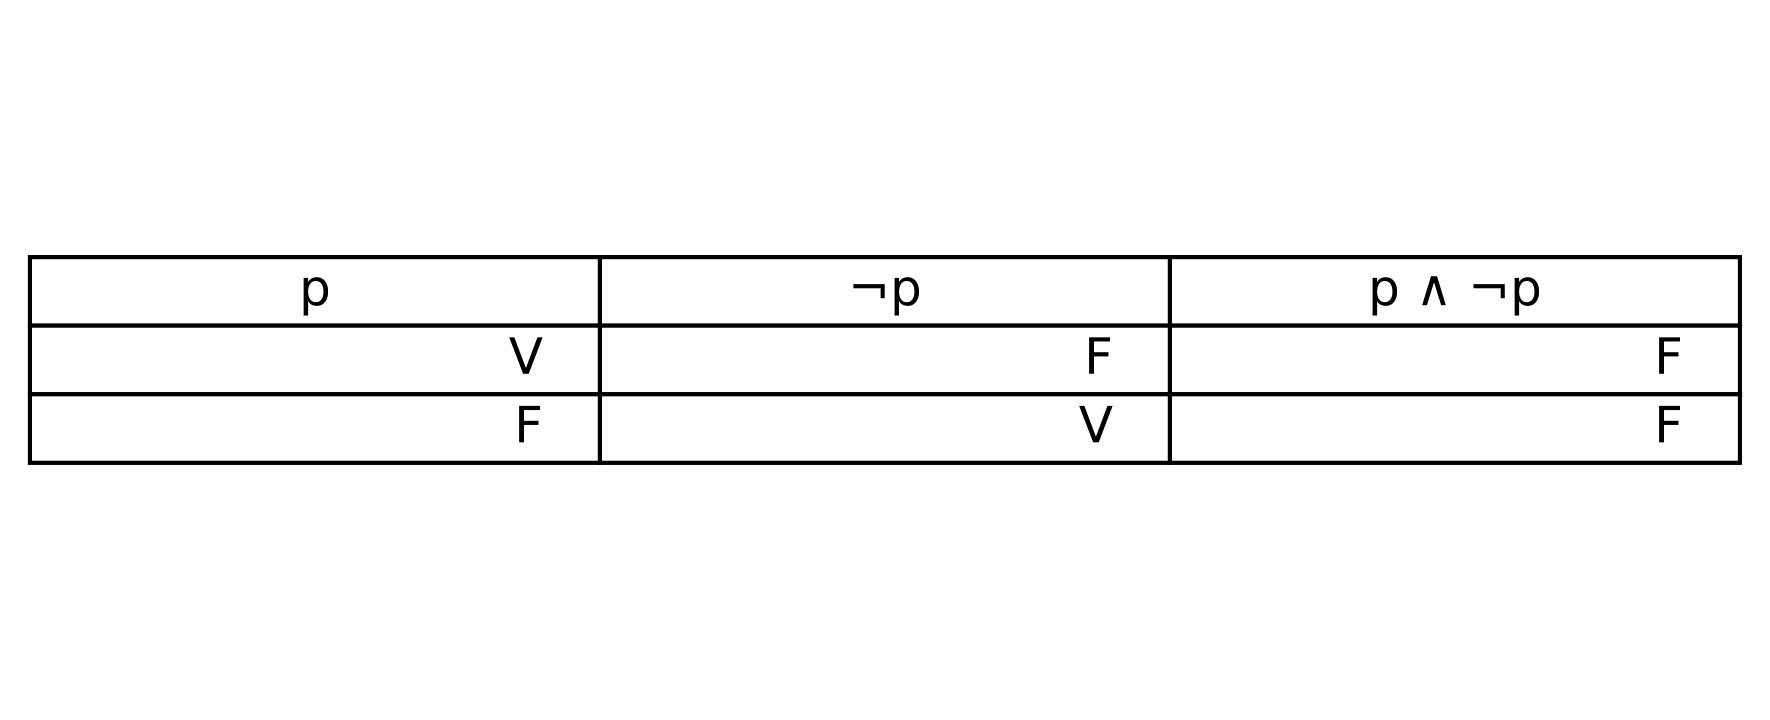
\includegraphics[height=0.3\textheight]{../assets/Talleres_fundamentos/ercicio_9_tabla_01.png}
  \end{center}

  \item $q \land \neg q$  
  \begin{center}
    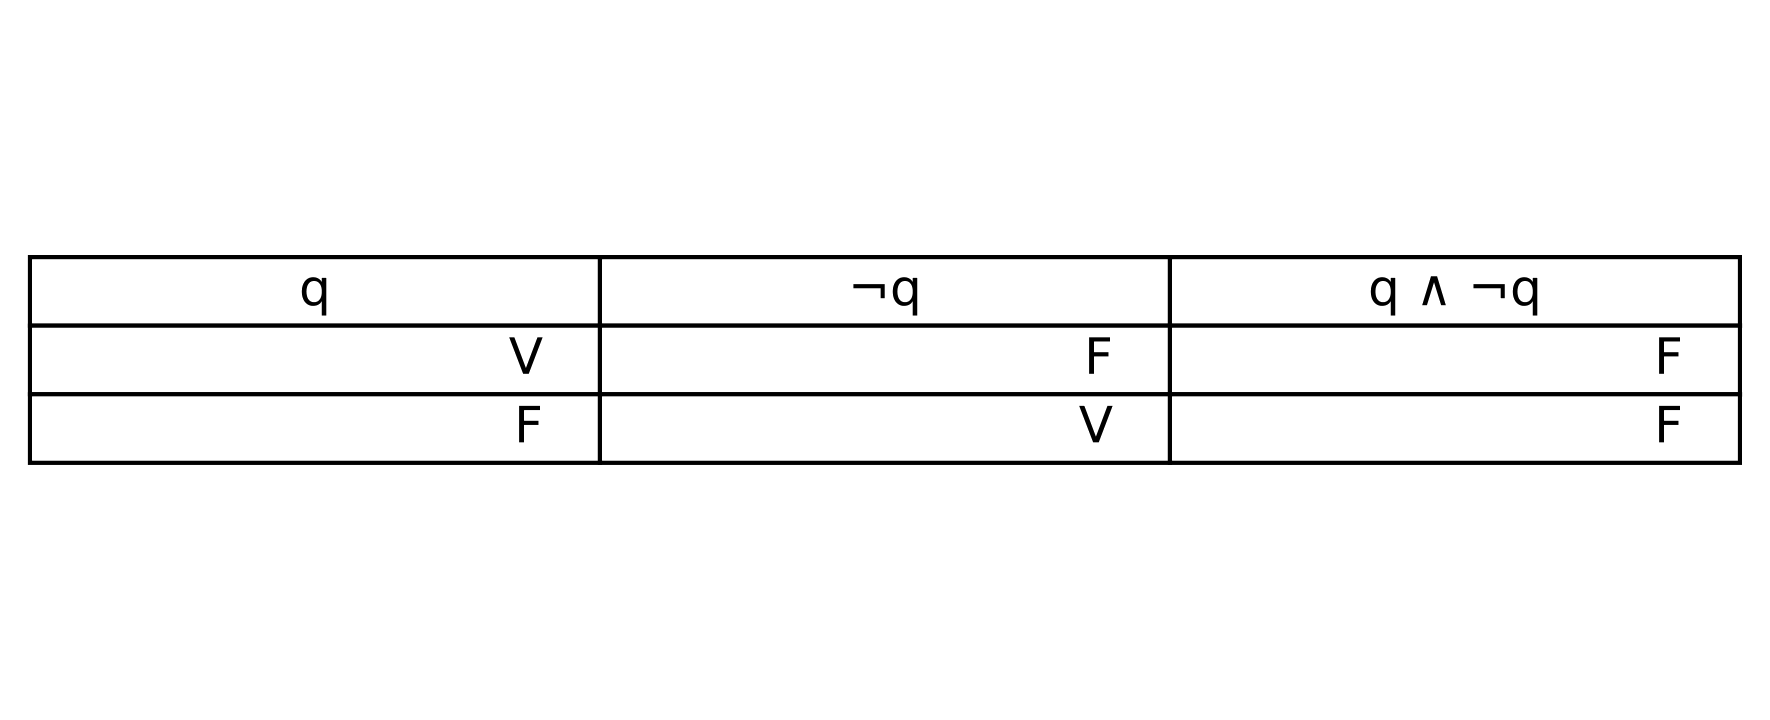
\includegraphics[height=0.3\textheight]{../assets/Talleres_fundamentos/ercicio_9_tabla_02.png}
  \end{center}

 \newpage
  \item $(p \lor q) \land \neg(p \lor q)$  
  \begin{center}
    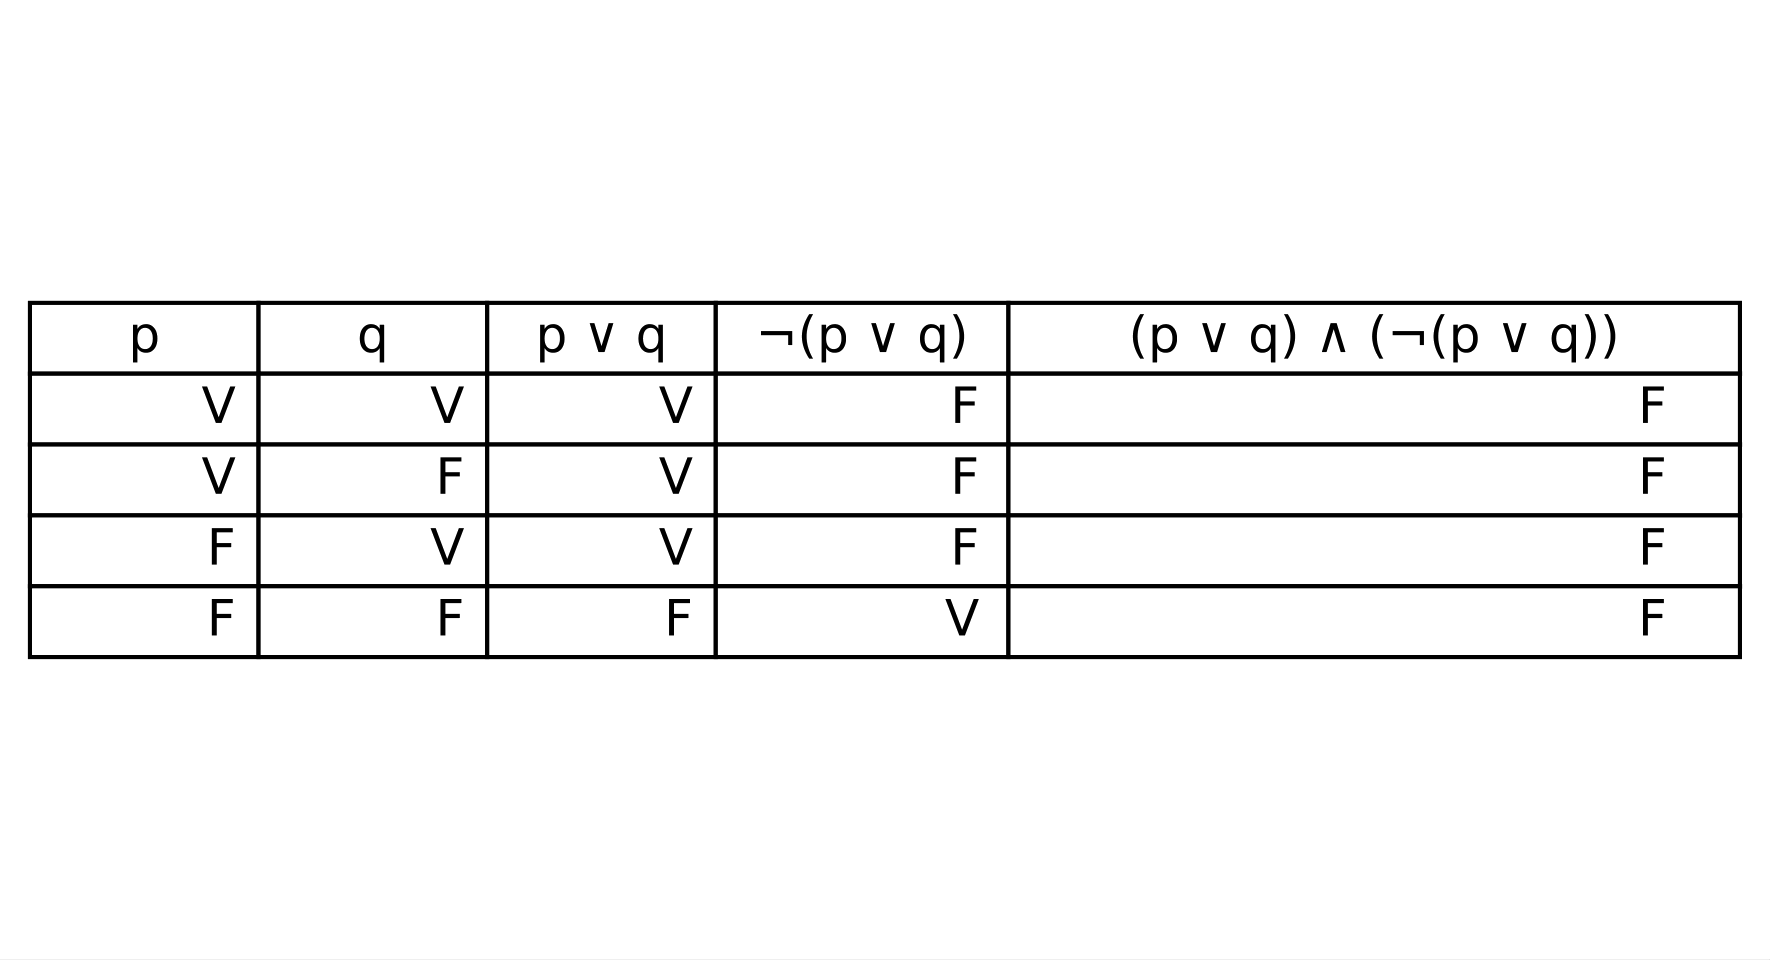
\includegraphics[height=0.3\textheight]{../assets/Talleres_fundamentos/ercicio_9_tabla_03.png}
  \end{center}

  \item $(p \land q) \land (\neg p \lor \neg q)$  
  \begin{center}
    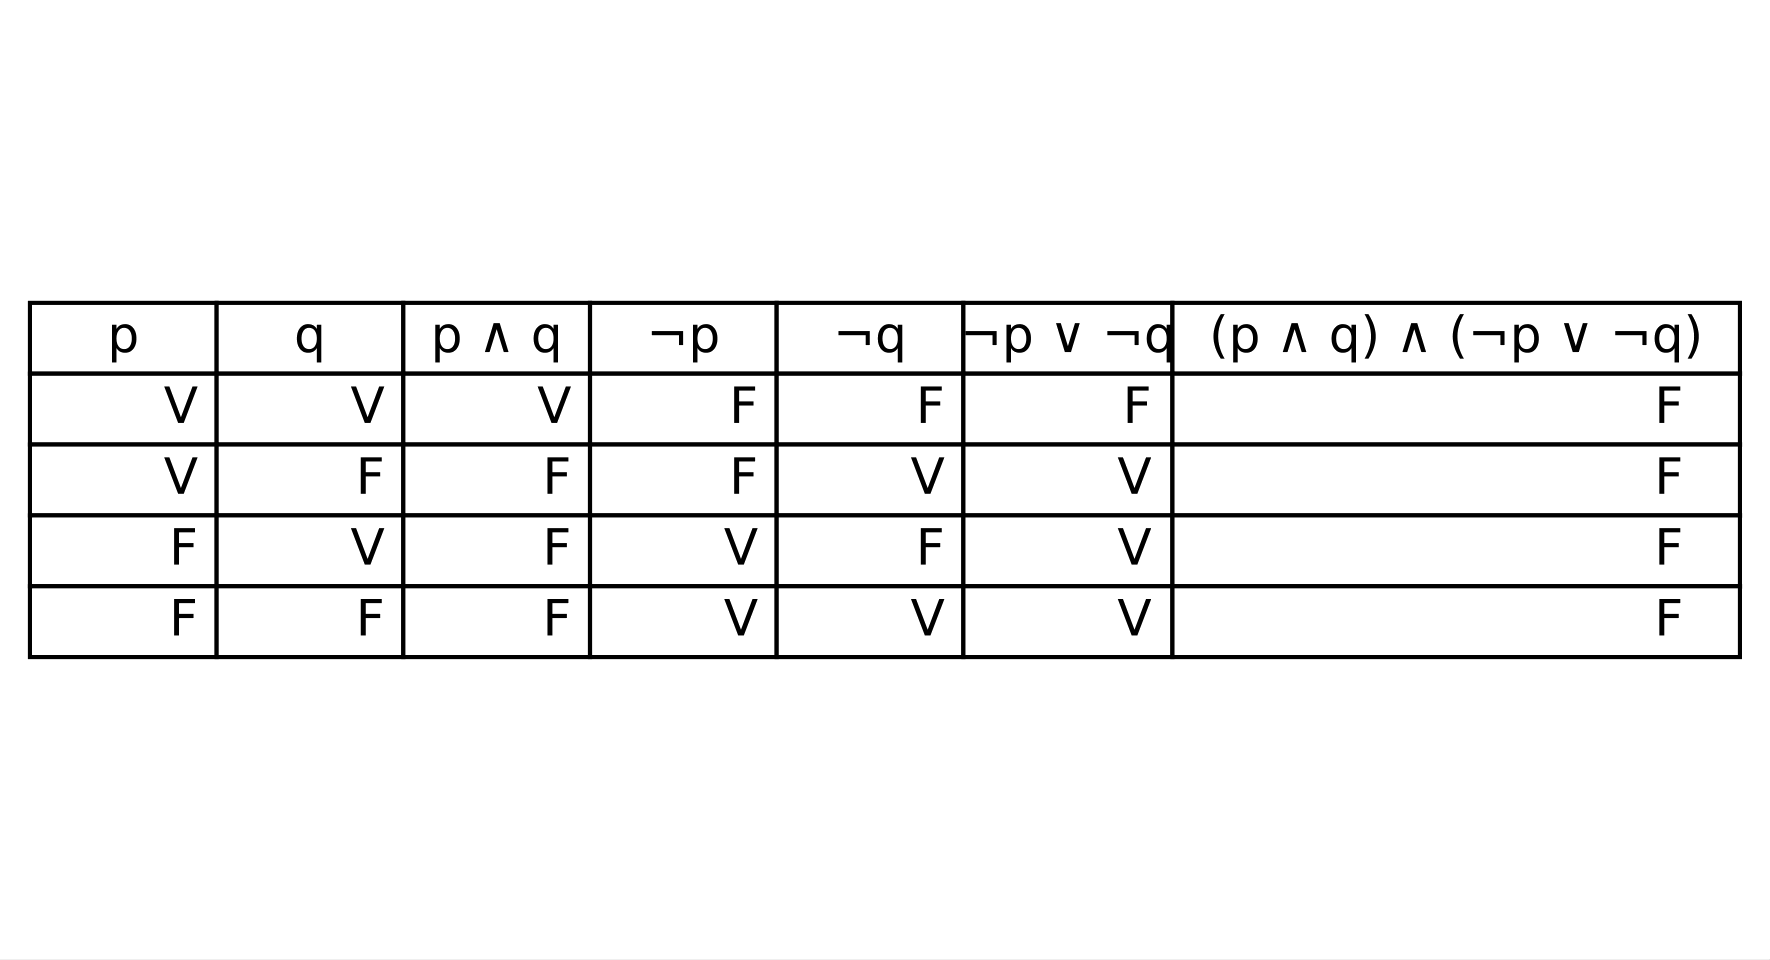
\includegraphics[height=0.3\textheight]{../assets/Talleres_fundamentos/ercicio_9_tabla_04.png}
  \end{center}
 \newpage
  \item $(p \rightarrow q) \land (p \land \neg q)$  
  \begin{center}
    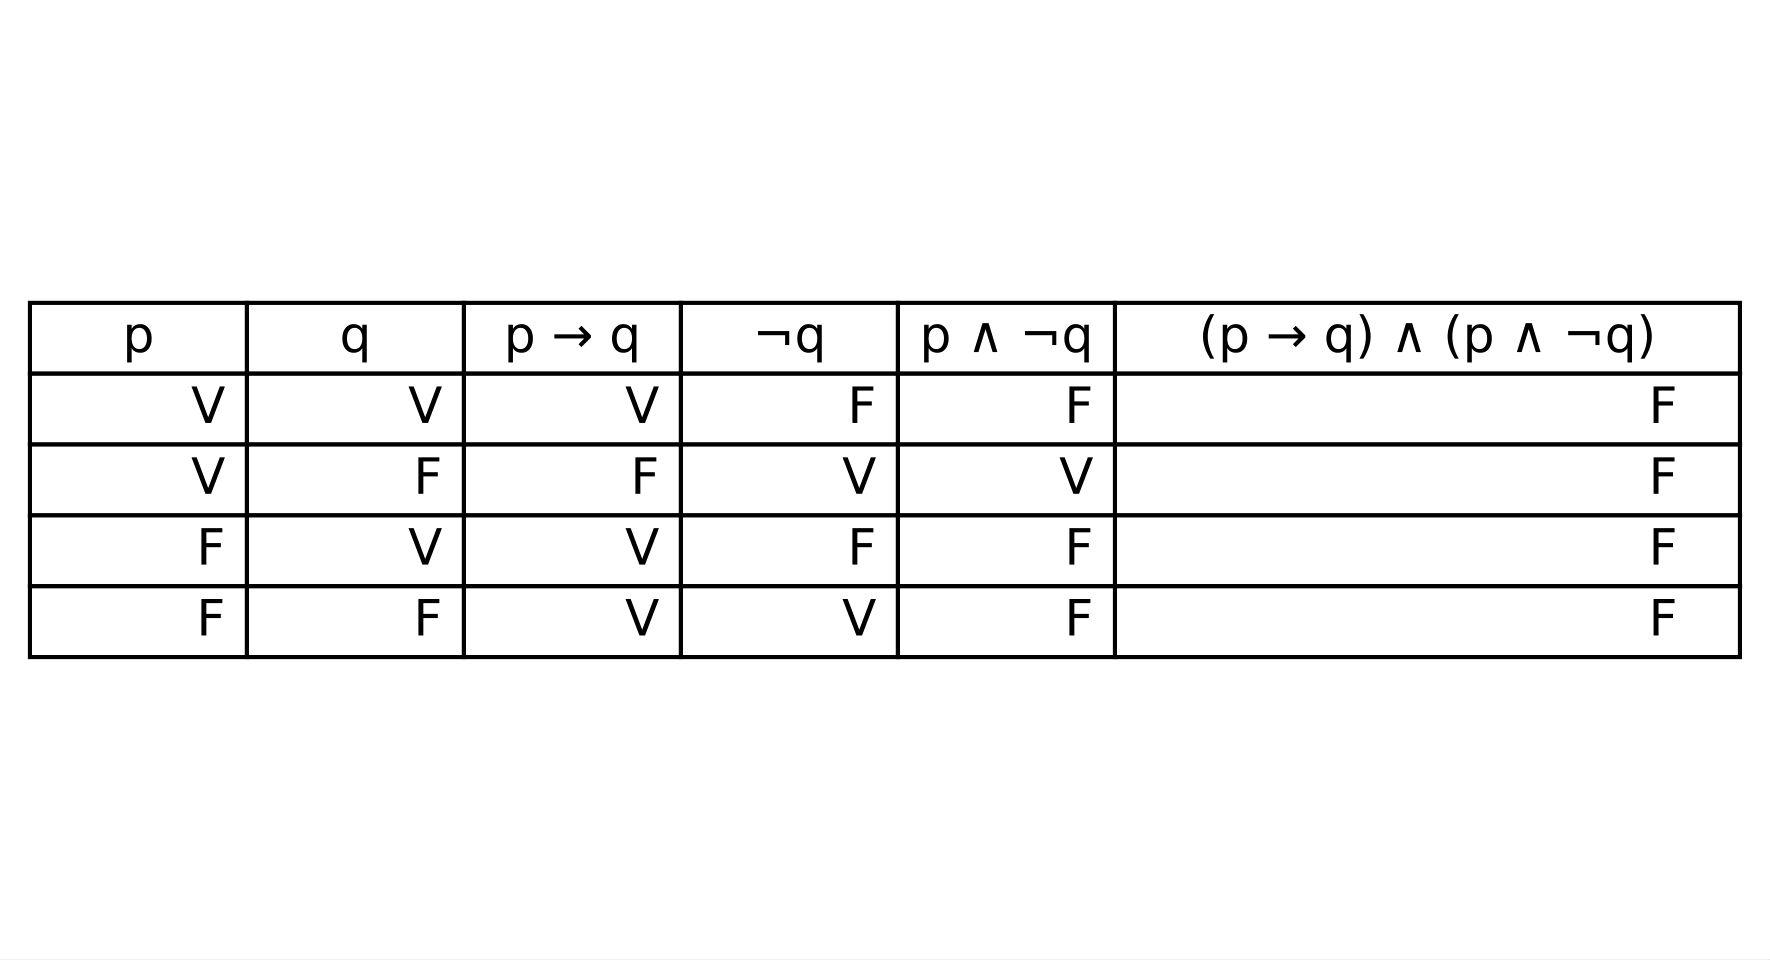
\includegraphics[height=0.3\textheight]{../assets/Talleres_fundamentos/ercicio_9_tabla_05.png}
  \end{center}
\end{enumerate}



\end{enumerate}


% \newpage % <-- separa visualmente los dos talleres
% ===== TALLER 2 =====
\section*{Taller 2}


\begin{enumerate}
  \item En los ejercicios, determine si el razonamiento es un ejemplo de razonamiento inductivo o deductivo..
  \begin{enumerate}[label=\alph*)]
  \item Si el mecánico dice que tardará siete días en reparar el automóvil de usted, entonces en realidad tardará 10 días. El mecánico dice: ``Calculo que tardaré una semana en arreglarlo''. Entonces usted espera que esté listo en 10 días a partir de ahora. 
  \\ Es \textbf{deductivo}, porque se pasa de un conocimiento general a uno particular \textcolor{ForestGreen}{(deductivo)}.

  \item Si usted toma sus vitaminas se sentirá mucho mejor. Usted toma sus vitaminas. Por lo tanto, se sentirá mucho mejor. 
  \\ Es \textbf{deductivo}, porque se pasa de un conocimiento general a uno particular \textcolor{ForestGreen}{(deductivo)}.

  \item Ha llovido todos los días durante los últimos seis días y también está lloviendo ahora. Entonces también lloverá mañana. 
  \\ Es \textbf{inductivo}, porque se pasa de un conocimiento particular a uno general \textcolor{red}{(inductivo)}.

  \item Los primeros tres hijos de Carrie fueron varones. Si tiene otro bebé será varón. 
  \\ Es \textbf{inductivo}, porque se pasa de un conocimiento particular a uno general \textcolor{red}{(inductivo)}.

  \item Finley tiene 85 tarjetas coleccionables de béisbol. Su mamá le regaló 20 más en su cumpleaños. Por lo tanto, ahora tiene 105 tarjetas. 
  \\ Es \textbf{deductivo}, porque se pasa de un conocimiento general a uno particular \textcolor{ForestGreen}{(deductivo)}.

  \item Si se resta el mismo número de ambos lados de una ecuación verdadera, la nueva ecuación también es verdadera. Yo sé que $9+18=27$. Por lo tanto, $(9+18)-13=27-13$. 
  \\ Es \textbf{deductivo}, porque se pasa de un conocimiento general a uno particular \textcolor{ForestGreen}{(deductivo)}.

  \item Si lo construye, ellos vendrán. Usted lo construye. Por lo tanto, ellos vendrán. 
  \\ Es \textbf{deductivo}, porque se pasa de un conocimiento general a uno particular \textcolor{ForestGreen}{(deductivo)}.

  \item Todos los hombres son mortales. Sócrates es un hombre. Por lo tanto, Sócrates es mortal. 
  \\ Es \textbf{deductivo}, porque se pasa de un conocimiento general a uno particular \textcolor{ForestGreen}{(deductivo)}.

  \item Es un hecho que todos los estudiantes que asistieron a Delgado University fueron aceptados en el posgrado. Como estudio en Delgado, puedo esperar que me acepten en el posgrado. 
  \\ Es \textbf{deductivo}, porque se pasa de un conocimiento general a uno particular \textcolor{ForestGreen}{(deductivo)}.

  \item En los últimos 97 años ha florecido una planta exótica en Columbia cada verano, alternando flores amarillas con flores rojas. De modo que el verano las plantas dieron flores verdes, y me dicen que en este verano habrá flores amarillas. 
  \\ Es \textbf{inductivo}, porque se pasa de un conocimiento particular a uno general \textcolor{red}{(inductivo)}.

  \item En la secuencia 5, 10, 15, 20, 25, $\ldots$, el siguiente número más probable es 30. 
  \\ Es \textbf{inductivo}, porque se pasa de un conocimiento particular a uno general \textcolor{red}{(inductivo)}.
  \end{enumerate}

  \item  Use el método de Gauss para calcular cada suma:
 \begin{enumerate}[label=\alph*)]
  \item La suma de los primeros 200 números naturales es:
  \[
  S = \frac{200 \cdot (200+1)}{2} = \frac{200 \cdot 201}{2} = 20100
  \]

  \item La suma de los primeros 800 números naturales es:
  \[
  S = \frac{800 \cdot (800+1)}{2} = \frac{800 \cdot 801}{2} = 320400
  \]

  \item Para la suma de los primeros 17 números:
  \[
  S = \frac{17 \cdot (17+1)}{2} = \frac{17 \cdot 18}{2} = 153
  \]
  Como el número de términos es impar, se forman $8$ parejas que suman $18$, 
  y queda el término central $9$. Entonces:
  \[
  S = (8 \times 18) + 9 = 144 + 9 = 153
  \]
\end{enumerate}

  \item Acertijo de Einstein.
  
  	La respuesta a la pregunta \textit{``¿Quién es el dueño del pececillo?''} es el 
  	\textbf{alemán}, ya que como se ve en las imágenes posteriores, es la única casilla en 
  	blanco.  
	
  	El procedimiento seguido fue el siguiente:  
	
  	Primero se listaron todas las variables del enunciado (nacionalidad, color de la casa, 
  	mascota, bebida y cigarrillo) y se organizaron en tablas. A partir de allí, se fueron 
  	marcando en las casillas las condiciones dadas directamente por el enunciado, y luego 
  	se fueron deduciendo las restricciones implícitas.  
	
  	En las tablas, las \textcolor{ForestGreen}{casillas verdes} representan coincidencias 
  	correctas que cumplen con las condiciones, mientras que las \textcolor{red}{casillas rojas} 
  	indican restricciones o imposibilidades.  
	
  	Mediante este proceso iterativo de \textbf{descartar posibilidades} e ir 
  	\textbf{confirmando coincidencias}, se fueron completando poco a poco las tablas. 
  	De esta manera, se logró reducir el problema hasta que únicamente quedó libre la 
  	casilla correspondiente al \textbf{alemán con el pez}, lo que permite concluir que él 
  	es el dueño del pececillo.  

  	%%%%%%%%%%%%%%%%%%%%%%%%%%%%%%%%%%%%%%%%%%%%%%%%%%%%%%%%%%%%%%%%%%%%%


\begin{center}
  
\Large\textbf{Acertijo de Einstein}\par
  \vspace{8mm}

  % Primera parte
  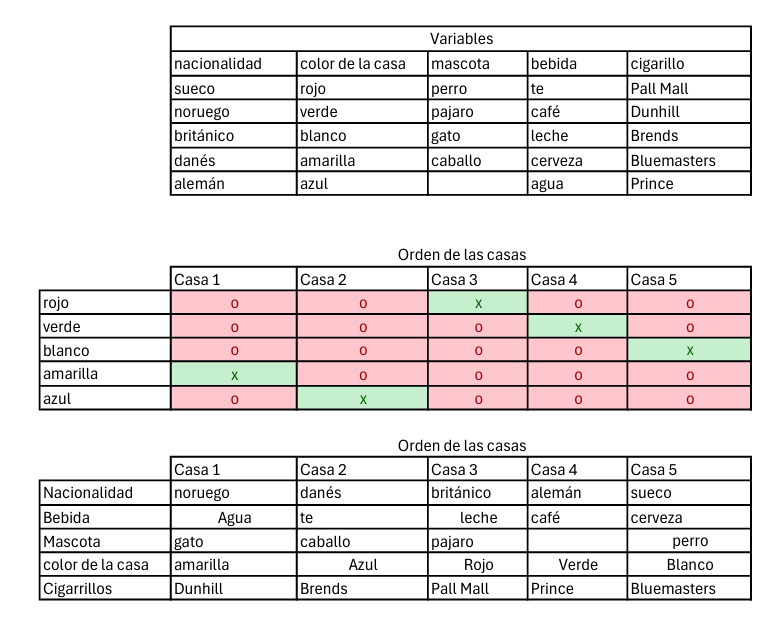
\includegraphics[width=\textwidth,keepaspectratio]{../assets/Talleres_fundamentos/Asertijo_Eintein_1.png}

  \vspace{1cm} % espacio entre las dos imágenes

  % Segunda parte
  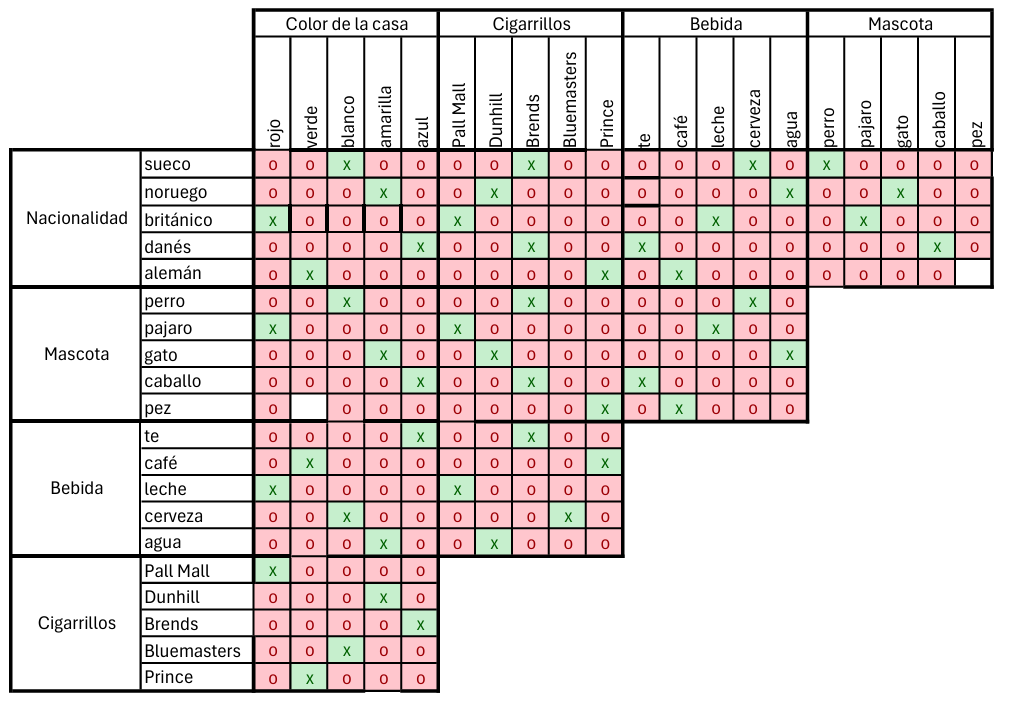
\includegraphics[width=\textwidth,keepaspectratio]{../assets/Talleres_fundamentos/Asertijo_Eintein_2.png}
\end{center}
 %%%%%%%%%%%%%%%%%%%%%%%%%%%%%%%%%%%%%%%%%%%%%%%%%%%%%%%%%%%%%%%%%%%%%%

  \item Explique cómo el siguiente diagrama ilustra geométricamente la fórmula
  \[
	1+3+5+7+9 = 25 = 5^2.
  \]
  \begin{center}
	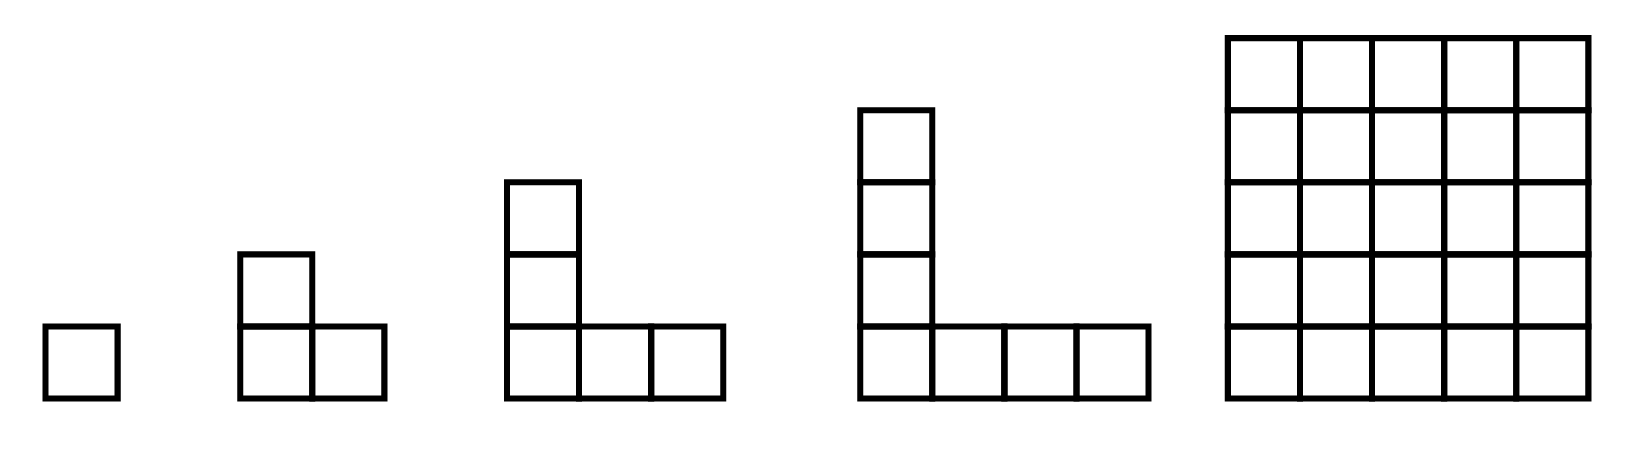
\includegraphics[width=0.5\textwidth]{../assets/Talleres_fundamentos/Taller2_imagen1.png}
  \end{center}
  	
	\vspace{1em}
 	\textcolor{ForestGreen}{Respeusta:} 

	El diagrama muestra que al sumar los primeros cinco números impares 
	\[
	1+3+5+7+9,
	\]
	podemos formar un cuadrado de lado $5$. Cada bloque en forma de ``L'' que aparece 
	en la construcción añade un número impar de cuadros, y al final todos juntos 
	completan un cuadrado de $5 \times 5$. 

	De esta manera se ilustra geométricamente que
	\[
	1+3+5+7+9 = 25 = 5^2.
	\]


  \item Explique cómo el siguiente diagrama ilustra geométricamente la fórmula
  	\begin{center}
		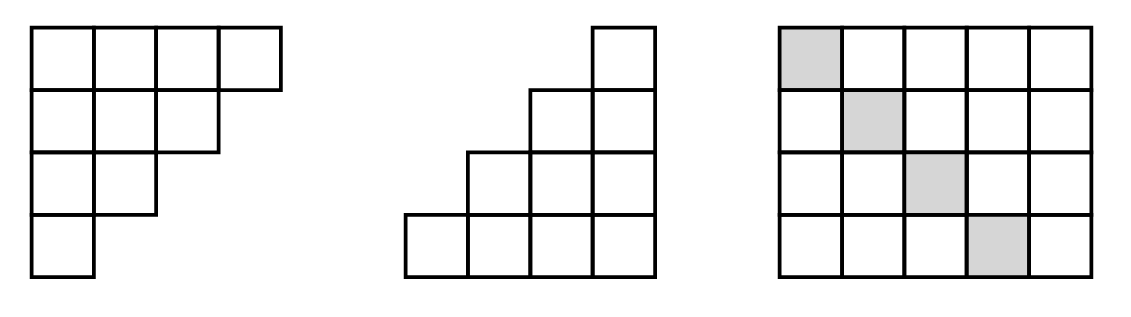
\includegraphics[width=0.5\textwidth]{../assets/Talleres_fundamentos/Taller2_imagen2.png}
  	\end{center}

  	\vspace{1em}
  	\textcolor{ForestGreen}{Respeusta:} 

  	El diagrama muestra que la suma
  	\[
  	1+2+3+4
  	\]
  	se puede interpretar como un triángulo rectángulo formado al apilar filas de 
  	cuadros. Si duplicamos este triángulo (colocando otra copia reflejada a lo largo 
  	de su diagonal), obtenemos un rectángulo de lados $4$ y $5$. 

  	El área del rectángulo es
  	\[
  	4 \times 5 = 20,
  	\]
  	pero como nuestro triángulo representa solo la mitad, su área (o número de cuadros)
  	es
  	\[
  	\frac{4 \times 5}{2} = 10.
  	\]

  	De esta forma, el diagrama ilustra geométricamente que
  	\[
  	1+2+3+4 = \frac{4 \times 5}{2}.
  	\]


  \item Indique si es válido o inválido cada uno de los siguientes argumentos.
  
  
\begin{enumerate}[label=\alph*)]

% a) Universal Orlando
\item Todos los parques de diversiones tienen recorridos emocionantes, Universal Orlando es un parque de diversiones, Universal Orlando tiene recorridos emocionantes.
\[
\begin{array}{c}
p \to q \\
p \\
\hline
q
\end{array}
\]
\begin{description}
  \item[$p$] es un parque de diversiones
  \item[$q$] tiene recorridos emocionantes
\end{description}

El argumento es del tipo \textbf{Modus Ponens} y es \textcolor{ForestGreen}{válido}.

% b) Disc jockeys
\item Todos los disc jockeys tocan música, Phlash Phelps es disc jockey, Phlash Phelps toca música.
\[
\begin{array}{c}
p \to q \\
p \\
\hline
q
\end{array}
\]
\begin{description}
  \item[$p$] es disc jockey
  \item[$q$] toca música
\end{description}

El argumento es del tipo \textbf{Modus Ponens} y es \textcolor{ForestGreen}{válido}.

% c) Políticos
\item Todos los políticos mienten, engañan y roban, ese hombre miente, engaña y roba, ese hombre es un político.
\[
\begin{array}{c}
p \to q \\
q \\
\hline
p
\end{array}
\]
\begin{description}
  \item[$p$] es político
  \item[$q$] miente, engaña y roba
\end{description}

El argumento es del tipo \textbf{Falacia del converso} y es \textcolor{red}{inválido}.

% d) Sureños
\item Todos los sureños hablan con acento, Bill Leonard habla con acento, Bill Leonard es sureño.
\[
\begin{array}{c}
p \to q \\
q \\
\hline
p
\end{array}
\]
\begin{description}
  \item[$p$] es sureño
  \item[$q$] habla con acento
\end{description}

El argumento es del tipo \textbf{Falacia del converso} y es \textcolor{red}{inválido}.

% e) Perros
\item A todos los perros les gusta enterrar huesos, a Puddles no le gusta enterrar huesos, Puddles no es un perro.
\[
\begin{array}{c}
p \to q \\
\neg q \\
\hline
\neg p
\end{array}
\]
\begin{description}
  \item[$p$] es un perro
  \item[$q$] le gusta enterrar huesos
\end{description}

El argumento es del tipo \textbf{Modus Tollens} y es \textcolor{ForestGreen}{válido}.

% f) Vicepresidentes
\item Todos los vicepresidentes usan teléfonos celulares, Bob DeBiasio no usa teléfono celular, Bob DeBiasio no es vicepresidente.
\[
\begin{array}{c}
p \to q \\
\neg q \\
\hline
\neg p
\end{array}
\]
\begin{description}
  \item[$p$] es vicepresidente
  \item[$q$] usa teléfono celular
\end{description}

El argumento es del tipo \textbf{Modus Tollens} y es \textcolor{ForestGreen}{válido}.

% g) Minnesota
\item Todos los residentes de Minnesota saben cómo vivir en temperaturas gélidas, Jessica Rockswold sabe cómo vivir en temperaturas gélidas, Jessica Rockswold vive en Minnesota.
\[
\begin{array}{c}
p \to q \\
q \\
\hline
p
\end{array}
\]
\begin{description}
  \item[$p$] es residente de Minnesota
  \item[$q$] sabe vivir en temperaturas gélidas
\end{description}

El argumento es del tipo \textbf{Falacia del converso} y es \textcolor{red}{inválido}.

% h) Dinosaurios
\item Algunos dinosaurios fueron herbívoros, Danny fue herbívoro, Danny fue un dinosaurio.
\[
\begin{array}{c}
p \to q \\
q \\
\hline
p
\end{array}
\]
\begin{description}
  \item[$p$] es dinosaurio
  \item[$q$] es herbívoro
\end{description}

El argumento es del tipo \textbf{Falacia del converso} y es \textcolor{red}{inválido}.

% i) Filósofos
\item Algunos filósofos son distraídos, Nicole Mallon es filósofa, Nicole Mallon es distraída.
\[
\begin{array}{c}
p \to q \\
p \\
\hline
q
\end{array}
\]
\begin{description}
  \item[$p$] es filósofo
  \item[$q$] es distraído
\end{description}

El argumento es del tipo \textbf{Modus Ponens} y es \textcolor{ForestGreen}{válido}.

% j) Enfermeras
\item Algunas enfermeras usan uniformes azules, Dee Boyle es enfermera, Dee Boyle usa uniforme azul.
\[
\begin{array}{c}
p \to q \\
p \\
\hline
q
\end{array}
\]
\begin{description}
  \item[$p$] es enfermera
  \item[$q$] usa uniforme azul
\end{description}

El argumento es del tipo \textbf{Modus Ponens} y es \textcolor{ForestGreen}{válido}.

% k) Camiones
\item Algunos camiones tienen sistemas de sonido, algunos camiones tienen estantes con armamento, algunos camiones con sistemas de sonido tienen estantes con armamento.
\[
\begin{array}{c}
p \to q \\
p \to r \\
\hline
q \land r
\end{array}
\]
\begin{description}
  \item[$p$] es camión
  \item[$q$] tiene sistema de sonido
  \item[$r$] tiene estantes con armamento
\end{description}

El argumento es del tipo \textbf{Falacia de composición} y es \textcolor{red}{inválido}.

\begin{center}
    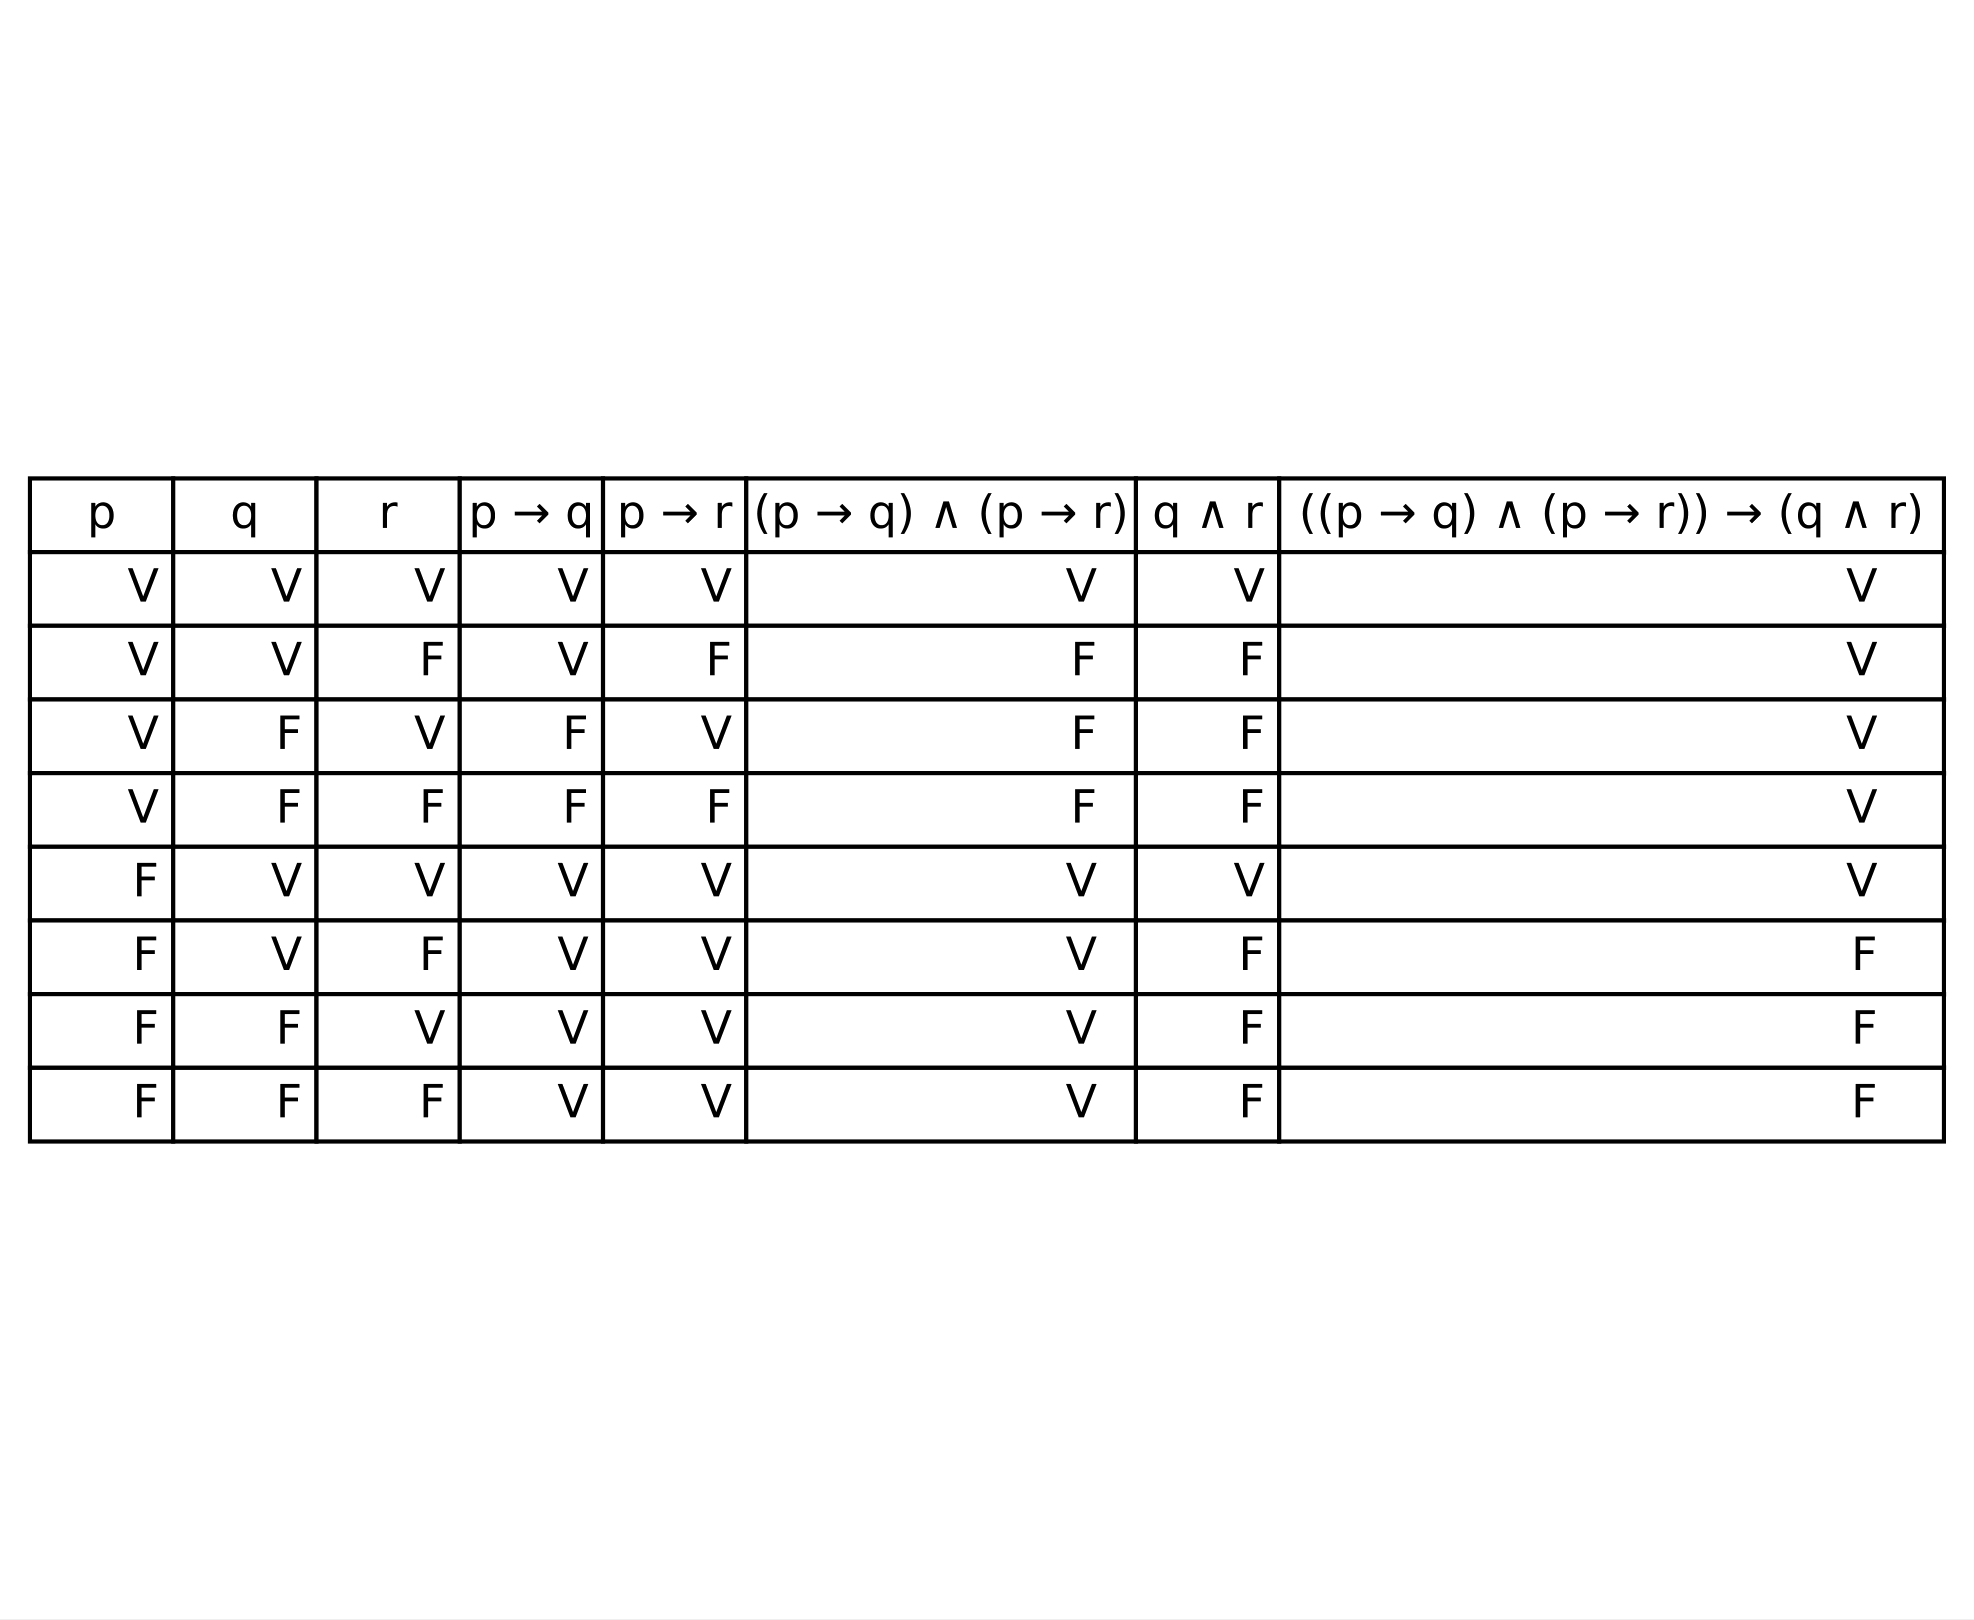
\includegraphics[height=0.4\textheight]{../assets/Talleres_fundamentos/Taller2_ejercicio_k.png}
  \end{center}

\end{enumerate}


\end{enumerate}

\end{document}
